\input{contents/header}

% \iccvfinalcopy % *** Uncomment this line for the final submission

\def\cvprPaperID{0008} % *** Enter the cvpr Paper ID here
\def\httilde{\mbox{\tt\raisebox{-.5ex}{\symbol{126}}}}

% Pages are numbered in submission mode, and unnumbered in camera-ready
\ifcvprfinal\pagestyle{empty}\fi

\begin{document}

%%%%%%%%% TITLE
\title{Supplementary Material \\ Estimating Correspondences of Deformable Objects ``In-the-wild"}
\author{Yuxiang Zhou \and Epameinondas Antonakos \and Joan Alabort-i-Medina \and Anastasios Roussos \and Stefanos Zafeiriou\\
Department of Computing, Imperial College London\\
180 Queen’s Gate, SW7 2AZ, London, U.K.\\
{\tt\small \{yuxiang.zhou10, e.antonakos, ja310, troussos, s.zafeiriou\}@imperial.ac.uk}}
\maketitle
\thispagestyle{empty}


%%%%%%%%% Appendix
\section*{Introduction}
In this supplementary material, we provide additional algorithmic details for our shape flow estimation, as well as additional visualizations and evaluations for the dense and patch-based AAMs that were constructed using the proposed framework.

%experimental evaluations for constructing both Dense AAMs and Patch-based AAMs using the proposed pipeline.
%For \textbf{Dense AAM}, We present more detailed algorithms explanation and intrinsic property analysis of Dense AAMs. In section~\ref{sec:cost_function},  minimisation of the energy function are described in more details. In Section \ref{sec:daam_fittingresults}, we present visualisations of in-the-wild model fitting  for faces and ears, comparing classic AAMs and the proposed dense AAMs. In Section \ref{sec:modelanalysis}, we provide evaluations and comparisons of dAAMs, in terms of model compactness, warping quality and reconstruction accuracy.
%For \textbf{Patch-based AAM}, we described how sparse landmark points are sparsely sampled from dense reference shape and mapped to rest shapes according to dense correspondences in section~\ref{sec:sparsesample}. A visualisation for Patch-based AAM shape model is presented in section~\ref{sec:paam_sm}. Also more visualisation of fitting results are shown in section~\ref{sec:paam_fittingresults}.



\appendix
\section{Implementation of Shape Flow Estimation}
\label{sec:cost_function}

As mentioned in the main submission (Section 3, Step 3), we propose to estimate the shape flow by minimizing the following energy:
\vspace{-5pt}
\begin{align}
E_{sf} & =\alpha
\int_{\Omega}\sum_{n=1}^{N_t} \|\bm{d}(\bx+\bm{u}_n(x);n)-\bm{d}(x;0)\| \ud \bx \label{eq:costfunc}\\
    &+ \beta \int_{\Omega}\sum_{n=1}^{N_t}\|\bm{u}_n(\bx)-\sum_{i=1}^R\bm{q}_i(n)\bm{v}_i(\bx)\|^2 \ud \bx \label{eq:lowrank}\\
    &+
\int_\Omega  \sum_{i=1}^R \,\, \left \|    \nabla \bm{v}_i(\bx)    \right \|  \,\ud \bx \label{eq:TVterm}
\vspace{-5pt}
\end{align}
We minimize this energy jointly with respect to $\bm{u}_n(\bx)$ and $\bm{v}_i(\bx)$, which correspond to the
two sets of unknown shape flows.
We implement this minimization based on the optimization algorithm described in \cite{Garg:2013hu} and the relevant publicly available code \footnote{https://bitbucket.org/troussos/mfsf/downloads}.
However, we modify this algorithm so that, instead of initialising the coarse-to-fine and warping iterations with a zero flow, we use Thin Plate Splines (TPS) \cite{Bookstein1989} interpolation of the initial correspondence vectors described in Section 3, Step 2 of the main submission.
This yields a significantly better initial location of the highly-nonconvex objective function and improves the computational efficiency, since much less coarse-to-fine pyramids are needed.

Regarding more details on the optimization algorithm, 
in every coarse-to-fine and warping iteration, we use an initialization that comes from the previous iteration. We approximate the data term \eqref{eq:costfunc} by linearizing the SVS images $\bm{d}(\bx;n)$ around the initialization. After that, the energy becomes convex and we optimize it using alternating optimization w.r.t.~$\bm{v}_i(\bx)$ and $\bm{u}_n(\bx)$. The minimization w.r.t.~$\bm{v}_i(\bx)$ is decoupled for every coefficient $i$ and corresponds to Rudin-Osher-Fatemi Total Variation denoising \cite{rudin92}, which we solve efficiently by applying the first order primal-dual algorithm of \cite{Chambolle:Pock:JMIV2011}. The minimization w.r.t.~$\bm{u}_n(x)$ is decoupled for every pixel $\bx$ and every shape index $i$. This minimization is also implemented by applying the efficient primal-dual algorithm of \cite{Chambolle:Pock:JMIV2011}.



\section{Dense Active Appearance Modeling}
\label{sec:daam}

In this section, we report additional qualitative and quantitative evaluations and comparisons for the dAAMs of faces and ears that were constructed using the proposed framework.



\subsection{Principal Components and Compactness}



Figure \ref{fig:pcamodel} visualizes some of the shape and appearance principal components of the built dAAMs for ears and faces. We observe that in both ears and faces, the variation of both shape and appearance captured by the model seem plausible.


\begin{figure*}[!t]
\centering
\includegraphics[width=\textwidth]{Suplementory_Meterial/Models/models}
\caption{Principal components of dAAMs built on ears (top) and faces (bottom). The mean (middle columns) as well as the first five principal components are visualised for both shape (left) and appearance (right). $\pm 3$ times the variance of the corresponding component is used in each case.}
\label{fig:pcamodel}
\end{figure*}


Figure \ref{fig:compact} shows the compactness plot for our dAAM for faces and compares it with the corresponding plot for a standard sparse AAM built on the same data. Note that these are the two shape models that are compared in Figure 9-left of the main submission. We observe that our dAAM is significantly more compact than the sparse AAM, since for any given number of components, it manages to explain a larger portion of the corresponding total variance of the training set. 


\begin{figure}[!b]
    \centering
%    \begin{subfigure}[b]{0.43\textwidth}
%            \includegraphics[width=\textwidth]{Suplementory_Meterial/Model_Analysis/var_ratio}
%        %\caption{dAAMs vs AAMs Variance Ratio}
%    \end{subfigure}
    \begin{subfigure}[b]{0.43\textwidth}
            \includegraphics[width=\textwidth]{Suplementory_Meterial/Model_Analysis/cumu_var_ratio}
        %\caption{dAAMs vs AAMs Cumulative Variance Ratio}
    \end{subfigure}
    \caption{Compactness plots of dAAM (green) and sparse AAM (blue) models for faces. Portion of the corresponding total variance explained as a function of the number of retained principal components.}
    \label{fig:compact}
\end{figure}

\subsection{Dense Shape Reconstruction Ability}

Figure \ref{fig:rc_face} evaluates the dense shape reconstruction ability of the proposed dAAMs and compares it with that of standard sparse AAMs. In more detail, we use shapes with dense 
ground-truth annotations and we use both AAMs and dAAMs to reconstruct them, by projecting on the corresponding model subspace. In the case of AAMs, which only contain a sparse shape model, we densify it using a piecewise affine transformation, which is typically used in texture warping textures using this type of models. We observe that dAAMs significantly outperform classic AAMs, in terms of dense shape reconstruction accuracy.

\begin{figure}[!b]
    \centering
    % \vspace*{-0.1in}
    \begin{subfigure}[b]{0.43\textwidth}
            \includegraphics[width=\textwidth]{Suplementory_Meterial/Model_Analysis/sr_ear}
        %\caption{dAAMs dense shape reconstruction}
    \end{subfigure}
    \\
    \begin{subfigure}[b]{0.43\textwidth}
            \includegraphics[width=\textwidth]{Suplementory_Meterial/Model_Analysis/sr_face}
        %\caption{AAMs dense shape reconstruction}
    \end{subfigure}
    \caption{Dense shape reconstruction errors for ears (top) and faces (bottom), using AAMs (red) and dAAMs (blue). The average normalized dense point-to-point distance error is plotted as a function of the number of principal components of the model.}
    \label{fig:rc_face}
\end{figure}





\subsection{Dense Fitting Visualizations}
\label{sec:daam_fittingresults}


In this section,
we visualize some characteristic examples of fitting
dense Active Appearance Models that were built using the proposed framework.
These results are characteristic examples that come from the quantitative evaluations and comparisons reported in Section 4.1 (``Non-rigid object alignment in-the-wild'') of the main submission. Figure \ref{fig:fr} shows dAAM fitting results using a grid visualisation, for both faces and ears. We observe that the proposed method successfully captures the shape deformations of these object classes and provides a detailed shape estimation for a variety of input images.


\begin{figure}[!t]
\centering
\includegraphics[width=0.5\textwidth]{Suplementory_Meterial/Fittings/fittings}
\caption{Examples of fitting
dAAMs that are constructed with the proposed pipeline. Results of dense fitting on images of
 ears (first two rows) and faces (last two rows). A grid visualisation is used.}
\label{fig:fr}
\end{figure}




\section{Patch-based Active Appearance Modeling}
\label{sec:paam}

In this section, we present additional visualizations and evaluations for the patch-based Active Appearance Model (PAAM) of arms that was constructed using the proposed framework.

\subsection{Subsampling of the Outline from Dense Correspondences}
\label{sec:sparsesample}

\begin{figure}[!b]
\centering
\newcommand{\ofh}{0.24\columnwidth}
    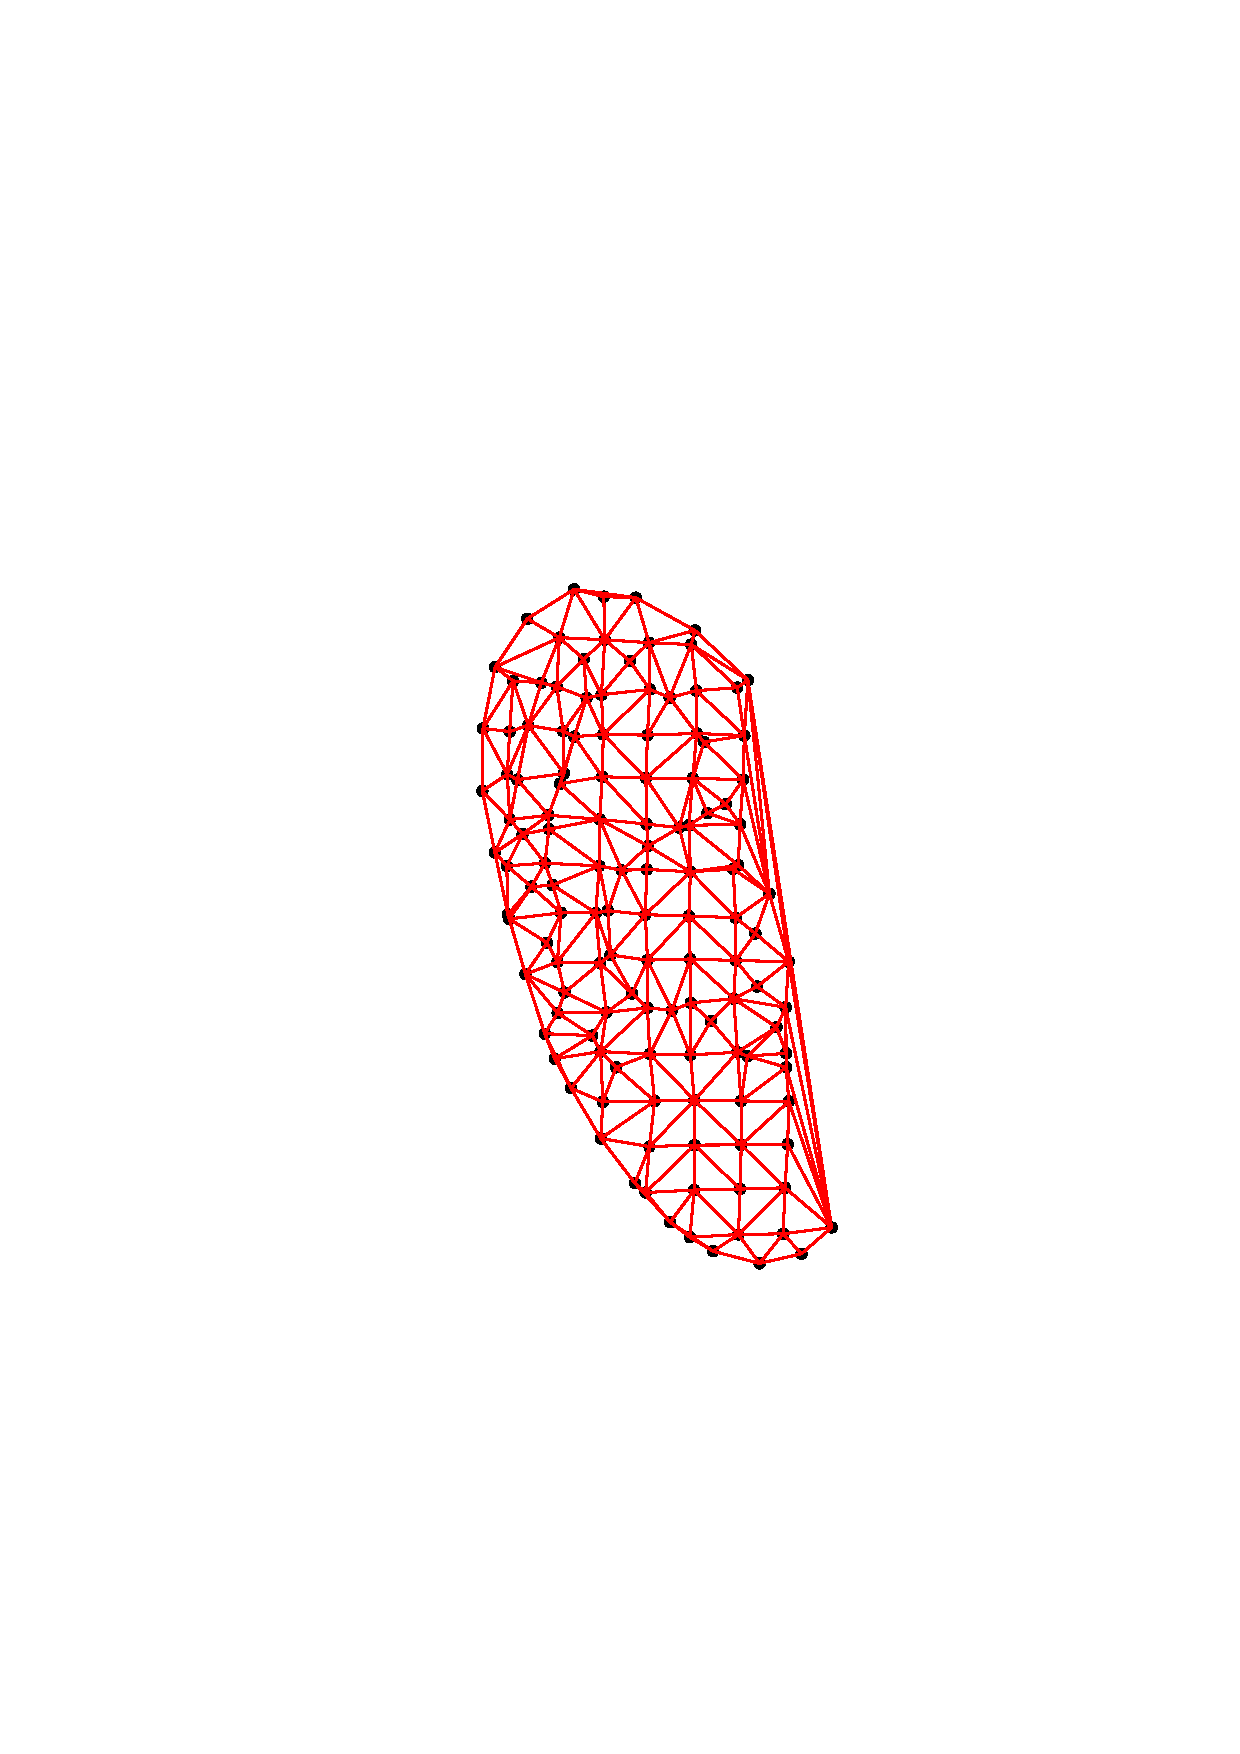
\includegraphics[height=\ofh]{Suplementory_Meterial/SparseSamples/mean.png}
    \hfill
    \includegraphics[height=\ofh]{Suplementory_Meterial/SparseSamples/mean-0.png}
    \hfill
    \includegraphics[height=\ofh]{Suplementory_Meterial/SparseSamples/mean-1.png}
    \hfill
    \includegraphics[height=\ofh]{Suplementory_Meterial/SparseSamples/mean-2.png}
    \hfill
    \includegraphics[height=\ofh]{Suplementory_Meterial/SparseSamples/mean-3.png}
    \hfill
    \includegraphics[height=\ofh]{Suplementory_Meterial/SparseSamples/mean-4.png}
\caption{Examples of sparse subsampling from dense shapes of arms. The dense correspondences (visualized via a deforming grid) are established using our shape flow estimation. The sparse landmarks (red dots) on the object outline are manually annotated only on the reference shape (left most image). In all other 5 example shapes, these landmarks have been automatically ``propagated'' using the established dense correspondences.}
\label{fig:sparsesample}
\end{figure}

As mentioned in the main submission (Section 3 - Step 4), in order to train a PAAM, we subsample the  densified training shapes to only consider points on the object outline. 
Some examples of this procedure are depicted in Figure~\ref{fig:sparsesample}. 
We manually annotate sparse outline points only on the reference shape. Then all other training shapes are subsampled automatically exploiting the dense correspondences that are established with our shape flow estimation. We observe that the automatic sub-sampling seems plausible, which is attributed to the accurate estimations of dense correspondences.


\subsection{Principal Components}
\label{sec:paam_sm}


    

Figure~\ref{fig:paam_sm} shows the mean shape and the first 4 principal components of shape variation of our PAAM for arms \footnote{Note that we do not visualize the appearance variation, since this is built using SIFT features and the corresponding 36-channel feature space cannot be visualized in an intuitive way.}. We observe that the shape variations captured by the model are plausible and seem to produce valid shapes of human arms.

\begin{figure}[!b]
\centering
\includegraphics[width=\columnwidth]{Suplementory_Meterial/HandSMPAAM/handsmpaam}
\caption{Principal components of our patch-based AAM for human arms.  The mean (left most column) as well as the first four principal components are visualised. $\pm 3$ times the variance of the corresponding component is used in each case.}
\label{fig:paam_sm}
\end{figure}





\subsection{Fitting Results}
\label{sec:paam_fittingresults}


Figure~\ref{fig:paam_fittingresults} demonstrates more fitting results produced by fitting patch-base AAM on arms datasets including MPII \cite{andriluka14cvpr}, Fashion Pose \cite{dantone2013human}, FLIC \cite{sapp2013modec} and BBC Poses \cite{pfister2015flowing}. All fittings are initialised using same method as mention in experiment 4.2 in main paper.


\begin{figure*}[!t]
    \newcommand{\ofh}{0.24\columnwidth}
    \centering
    \includegraphics[height=\ofh]{Suplementory_Meterial/ExFit/0001.eps}
    \hfill
    \includegraphics[height=\ofh]{Suplementory_Meterial/ExFit/0002.eps}
    \hfill
    \includegraphics[height=\ofh]{Suplementory_Meterial/ExFit/0003.eps}
    \hfill
    \includegraphics[height=\ofh]{Suplementory_Meterial/ExFit/0004.eps}
    \hfill
    \includegraphics[height=\ofh]{Suplementory_Meterial/ExFit/0005.eps}
    \hfill
    \includegraphics[height=\ofh]{Suplementory_Meterial/ExFit/0006.eps}
    \hfill
    \includegraphics[height=\ofh]{Suplementory_Meterial/ExFit/0007.eps}
    \hfill
    \includegraphics[height=\ofh]{Suplementory_Meterial/ExFit/0008.eps}
    \hfill
    \includegraphics[height=\ofh]{Suplementory_Meterial/ExFit/0009.eps}
    \hfill
    \includegraphics[height=\ofh]{Suplementory_Meterial/ExFit/0010.eps}
    \hfill
    \includegraphics[height=\ofh]{Suplementory_Meterial/ExFit/0011.eps}
    \hfill
    \includegraphics[height=\ofh]{Suplementory_Meterial/ExFit/0012.eps}
    \hfill
    \includegraphics[height=\ofh]{Suplementory_Meterial/ExFit/0013.eps}
    \hfill
    \includegraphics[height=\ofh]{Suplementory_Meterial/ExFit/0014.eps}
    \hfill
    \includegraphics[height=\ofh]{Suplementory_Meterial/ExFit/0015.eps}
    \hfill
    \includegraphics[height=\ofh]{Suplementory_Meterial/ExFit/0017.eps}
    \hfill
    \includegraphics[height=\ofh]{Suplementory_Meterial/ExFit/0018.eps}
    \hfill
    \includegraphics[height=\ofh]{Suplementory_Meterial/ExFit/0019.eps}
    \hfill
    \includegraphics[height=\ofh]{Suplementory_Meterial/ExFit/0020.eps}
    \hfill
    \includegraphics[height=\ofh]{Suplementory_Meterial/ExFit/0021.eps}
    \hfill
    \includegraphics[height=\ofh]{Suplementory_Meterial/ExFit/0022.eps}
    \hfill
    \includegraphics[height=\ofh]{Suplementory_Meterial/ExFit/0023.eps}
    \hfill
    \includegraphics[height=\ofh]{Suplementory_Meterial/ExFit/0024.eps}
    \hfill
    \includegraphics[height=\ofh]{Suplementory_Meterial/ExFit/0025.eps}
    \hfill
    \includegraphics[height=\ofh]{Suplementory_Meterial/ExFit/0026.eps}
    \hfill
    \includegraphics[height=\ofh]{Suplementory_Meterial/ExFit/0027.eps}
    \hfill
    \includegraphics[height=\ofh]{Suplementory_Meterial/ExFit/0028.eps}
    \hfill
    \includegraphics[height=\ofh]{Suplementory_Meterial/ExFit/0029.eps}
    \hfill
    \includegraphics[height=\ofh]{Suplementory_Meterial/ExFit/0030.eps}
    \hfill
    \includegraphics[height=\ofh]{Suplementory_Meterial/ExFit/0031.eps}
    \hfill
    \includegraphics[height=\ofh]{Suplementory_Meterial/ExFit/0032.eps}
    \hfill
    \includegraphics[height=\ofh]{Suplementory_Meterial/ExFit/0033.eps}
    \hfill
    \includegraphics[height=\ofh]{Suplementory_Meterial/ExFit/0034.eps}
    \hfill
    \includegraphics[height=\ofh]{Suplementory_Meterial/ExFit/0035.eps}
    \hfill
    \includegraphics[height=\ofh]{Suplementory_Meterial/ExFit/0036.eps}
    \hfill
    \includegraphics[height=\ofh]{Suplementory_Meterial/ExFit/0037.eps}
    \hfill
    \includegraphics[height=\ofh]{Suplementory_Meterial/ExFit/0038.eps}
    \hfill
    \includegraphics[height=\ofh]{Suplementory_Meterial/ExFit/0039.eps}
    \hfill
    \includegraphics[height=\ofh]{Suplementory_Meterial/ExFit/0040.eps}
    \hfill
    \includegraphics[height=\ofh]{Suplementory_Meterial/ExFit/0041.eps}
    \hfill
    \includegraphics[height=\ofh]{Suplementory_Meterial/ExFit/0042.eps}
    \hfill
    \includegraphics[height=\ofh]{Suplementory_Meterial/ExFit/0043.eps}
    \hfill
    \includegraphics[height=\ofh]{Suplementory_Meterial/ExFit/0044.eps}
    \caption{Demonstration of outline fitting of patch-based AAM on arms. Images are cropped to arms only for better visualisation.}
    \label{fig:paam_fittingresults}
\end{figure*}


In addition table~\ref{tab:hand_benchmark} presents statistics results that refers to experiment 4.2 in main paper for additional information. Column $\leq 6pt$ reports the percentage of fittings that having errors, point-to-point distance on normalised images, less than 6 pixels (same measurement used in \cite{pfister2015flowing}). This shows we have notable improvement on estimating wrists and comparable results on estimating elbow.


\begin{table}[t!]
    \small
    \centering
    \begin{tabular}{|l|c|c|c||c|c|c|}
        \hline
                            & \multicolumn{3}{c||}{Wrist} & \multicolumn{3}{c|}{Elbow}\\
        \hline
        \emph{Method}       & \emph{mean} & \emph{std} & $\leq 6pt$ & \emph{mean} & \emph{std} & $\leq 6pt$\\
        \hline\hline
        Buehler             & 12.08    & 19.94        & 44.5\%       & 12.94    & 14.65        & 34.4\%\\
        Charles14           & 11.81    & 20.89        & 54.2\%       &  8.30    & 11.00        & \textbf{55.2\%}\\
        Charles13           & 13.78    & 22.39        & 43.3\%       & 13.17    & 18.74        & 46.3\%\\
        Pfister14           & 14.69    & 17.89        & 29.7\%       & 14.60    & 10.59        & 14.0\%\\
        Ramanan             & 15.59    & 19.04        & 22.6\%       & 15.53    & 10.82        & 15.8\%\\
        Pfister15           & 7.62     & 11.04        & 54.1\%       &  8.84    & 11.44        & 54.9\%\\
        \hline\hline
        Ours                & \textbf{6.71}& \textbf{10.90}   & \textbf{63.1\%}       & \textbf{8.20}     &  \textbf{10.54}        & 52.1\%\\
        \hline
    \end{tabular}
    \caption{Fitting statistics on BBC Pose database for experiment 4.2 in main paper.}
    \label{tab:hand_benchmark}
\end{table}





{\small
\bibliographystyle{ieee}
\bibliography{bib}
}


\end{document}









% \subsection{Appearance Reconstruction}
% \label{sec:reconstruct}

% \begin{figure}[!b]
%     \centering
%     %\vspace*{-0.2in}
%     \includegraphics[width=0.5\textwidth]{Suplementory_Meterial/Fig_Draw/draw}
%     \caption{Synthesizing face images from caricature sketches. First column: caricature sketches. Second column: arbitrary chosen face images. Third and last column: sketch-based warping of images based on AAMs (third column) and dAAMs (last column).}
%     \label{fig:draw}
% \end{figure}

% In this qualitative experiment, we show how the proposed pipeline can be used to generate novel modified instances of an object, e.g. caricatures. To be specific, firstly we manually craft a set of hand-drawn cartoon-like shape sketches. We then apply shape flow to align them with the reference frame. In this way, we establish dense correspondences of landmarks. Afterwards, we perform shape reconstruction using both AAMs and dAAMs. Finally, we warp the appearance from arbitrarily chosen faces on the reconstructed shape using either piecewise affine warp (in the case of AAMs) or shape flow (in the case of dAAMs). The corresponding results are shown in figure \ref{fig:draw}. We see that AAMs introduce more severe artifacts, especially on the areas of mouth and eyes, where nuanced information is missing or models are overly deformed. In contrast, dAAMs yield a significantly more plausible result.



% \section{Segmentation using Dense AAM}
% \label{sec:segmentation}

% In this section, we present experiments of utilising our dense AAM for object segmentation. Two object classes, bottles and human bodies, are considered. For human bodies, we use images along with ground truth segmentation from Space-Time Actions dataset \footnote{\label{sta} \url{http://www.wisdom.weizmann.ac.il/~vision/SpaceTimeActions.html}}, which includes sequences with several human actions. We use ``jumping'' and ``sliding'' actions. As far as bottles are concerned, we use 500 high-resolution images that we collected and annotated using a newly-defined 50 point annotation scheme, as well as the curve annotations proposed in this paper. We randomly split these images into two disjoint sets of training (400) and testing (100) images. Bottle models were built using 400 training images while body models are built in terms of human actions (e.g. jumping), each having approximately 200 training images and 50 test images.

% \begin{figure}[!t]
%     \centering
%     \begin{subfigure}[b]{0.15\textwidth}
%             \includegraphics[height=\textwidth]{Suplementory_Meterial/Segmentation_Measure/ear}
%         %\caption{Ear Initial Bounding Box}
%     \end{subfigure}
%     \begin{subfigure}[b]{0.15\textwidth}
%             \includegraphics[height=\textwidth]{Suplementory_Meterial/Segmentation_Measure/bottle}
%         %\caption{Bottle Initial Bounding Box}
%     \end{subfigure}
%     \begin{subfigure}[b]{0.15\textwidth}
%             \includegraphics[height=\textwidth]{Suplementory_Meterial/Segmentation_Measure/body}
%         %\caption{Body Initial Bounding Box}
%     \end{subfigure}
%     \caption{Examples of fitting initialisations used for the segmentation experiment. These are created by random perturbation of the ground-truth bounding box.}
%     \label{fig:seg_init}
% \end{figure}

% Fitting dAAMs on test images yields dense landmarks that can be used to perform segmentation. In a real-world scenario, a simple object detector would be required to be applied prior to our pipeline to initialise the fitting. However, as a simple evaluation, we initialise the fitting by randomly perturbing the ground-truth bounding box with certain variance to simulate an object detector with implicit detection, see e.g.~Figure \ref{fig:seg_init}. Table  \ref{tab:seg_result} reports the segmentation precision, in case of fitting bottles and human bodies by adopting the proposed dAAMs pipeline.

% \begin{table}[!h]
% \small
% \centering
% \begin{tabular}{|l|c|c|c|}
% \hline
% \emph{Object}   & \emph{mean} & \emph{std} & \emph{median}\\
% \hline\hline
% Bottles         & 0.8125      & 0.1460     & 0.8414\\
% Action - Jump   & 0.6102      & 0.0198     & 0.6099\\
% Action - Slide  & 0.6444      & 0.0500     & 0.6501\\
% \hline
% \end{tabular}
% \caption{Segmentation precision, in case of fitting bottles and human bodies by adopting the proposed dAAMs pipeline. The mean, standard deviation and median of the precision error are provided.}
% \label{tab:seg_result}
% \end{table}